\subsection{Introduction}
\begin{key}{Datacenter}
A Datacenter is a building whose primary purpose is to house a computer 
room and its support areas, so that services can run continuously and 
efficiently
\end{key}
There exist lots of different types of datacenters:
\begin{itemize}
\item \textbf{Enterprise Data Centers} 
    - facilities operated and controlled by the company that provides the 
    service. Main problem: expensive to maintain (to build or not to 
    build dilemma) and can shorten the possibility to generate money by 
    the business.
\item \textbf{Colocation Data Centers} - 
    larger facilities built to accomodate different businesses and can
    personalize individual IT parts for individual businesses. 
    Main problem: IT purchases are on your own and restrictions 
    on access and maintenance. 
\item \textbf{Managed Hosting Platforms} - 
    all facilities are managed by third parties, still a single-tenant solution.
    Main problem: higher operational costs and possibility of customer 
    lock in problem.
\end{itemize}

In addition to the above solutions, there are also \textbf{Cloud Data Centers}, 
which are the most common solution in post-pandemic times. Those solutions
are \textbf{IaaS}, \textbf{PaaS} and \textbf{SaaS}. A clear representation is 
shown in the figure below.
\begin{figure}[H]
    \centering
    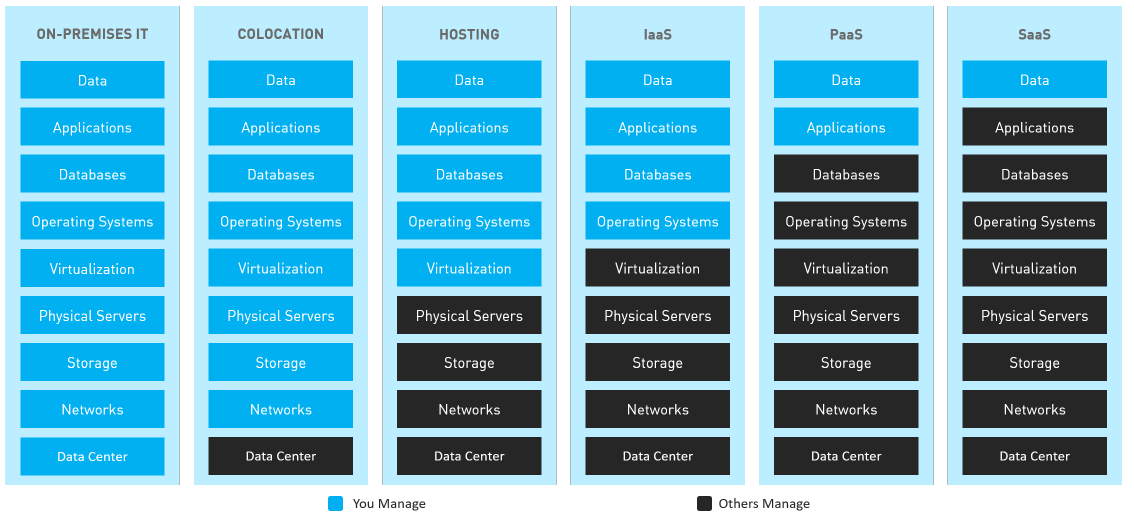
\includegraphics[width=0.8\textwidth]{Images/1DatacenterTypes.png}
    \caption{Cloud Data Centers}
    \end{figure}
One thing that stands out is that cloud solutions also contain virtualization 
managed by the provider (you don't know which operating system is running, 
you are inside an additional abstraction layer).

\subsection{Hardware Infrastructures}
Let's start with the basic definition of a computing infrastructure.
\begin{key}{Computing Infrastructure}
    A \textbf{Computing Infrastructure} is a tecnological infrastructure that 
    provides hardware and software for computation to other systems and services.
\end{key}
Computing infrastructures can be categorized in a pyramid of three layers:
\begin{itemize}
    \item \textbf{IoT and AI-enabled Edge Sensors} - 
    where data acquisition and processing happens at the edge of the network.
    \item \textbf{Edge Servers} - 
    on-premises hardware resources that perform more intensive processing tasks.
    \item \textbf{Data Centers and Cloud} -
    virtualized computing and capacity on demand.
\end{itemize}
\begin{figure}[h]
    \centering
    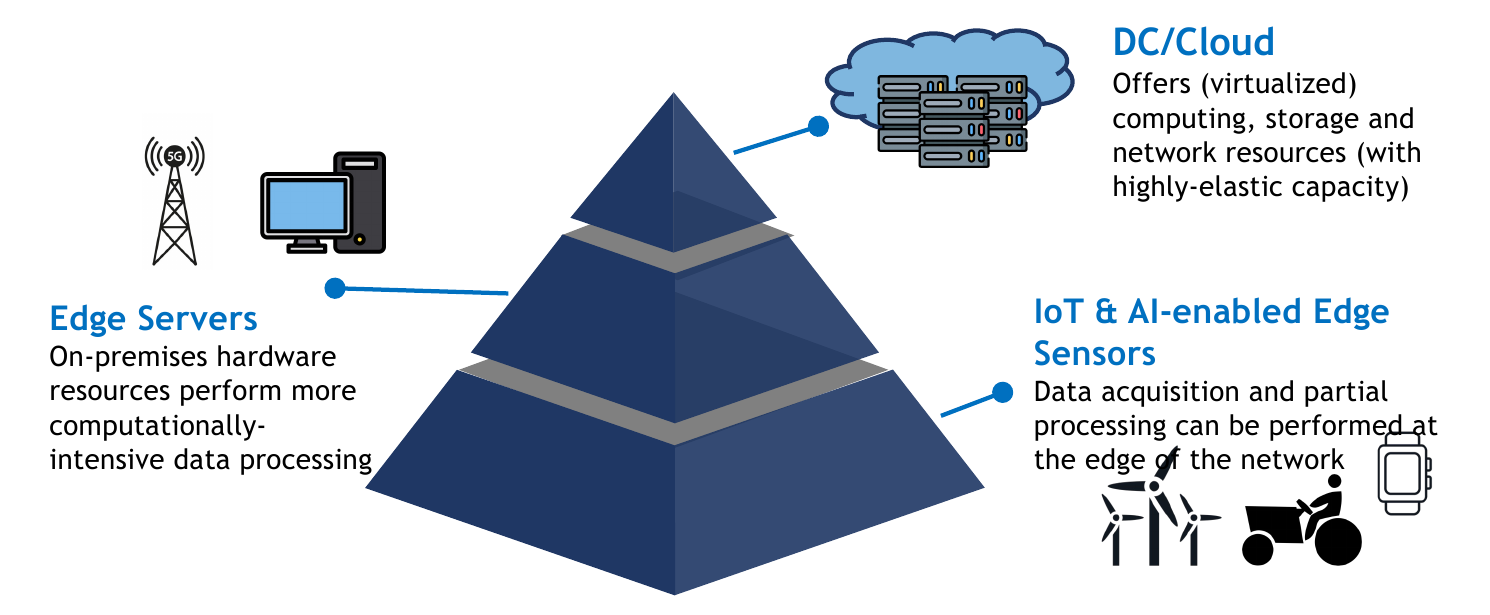
\includegraphics[width=0.8\textwidth]{Images/2ComputingInfrastructures.png}
    \caption{Computing Infrastructure Pyramid}
\end{figure}
It's obvious that the bottom layer has less memory and computational power,
but it is also more responsive and with low latency; the upper layers offer
more resources to work with. To categorize all the components of a system
it is used what is called the \textbf{Computing Continuum}.
\subsubsection{Data Centers}
\begin{figure}[h]
    \centering
    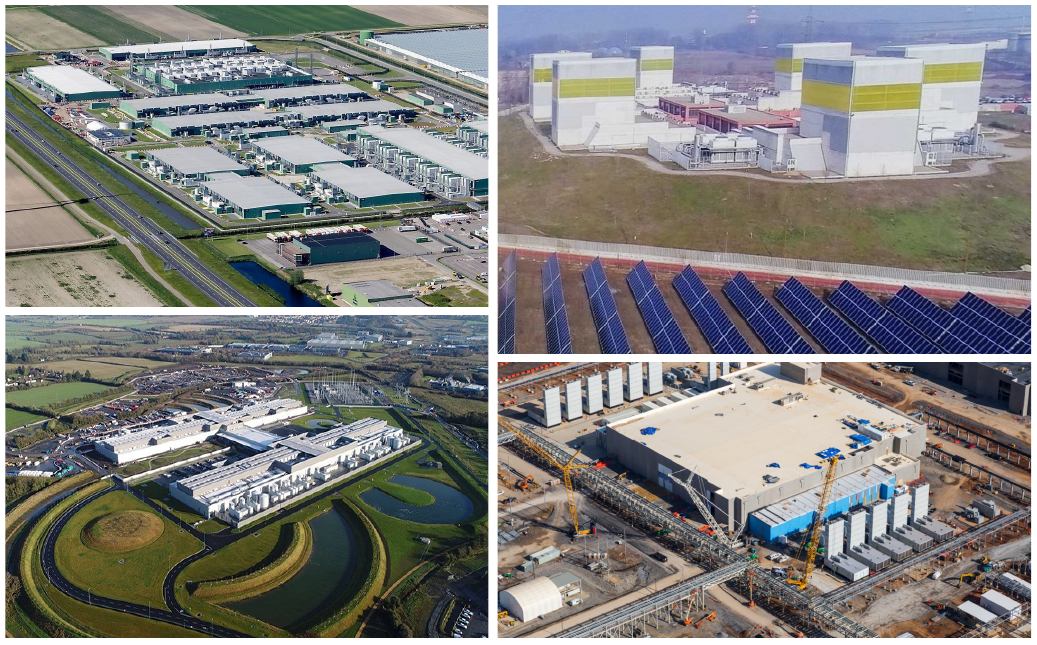
\includegraphics[width=0.8\textwidth]{Images/3DataCentersGeneric.png}
    \caption{Data Centers}
\end{figure}
Usually, data centers contain servers for \textbf{processing}, \textbf{storage}
and \textbf{communication}. They have lower IT costs, high performance, 
"unlimited" storage capacity, universal data access and have device
independence. On the other hand they need a constant internet connection, 
they do not work well with low speed connections, have high power consumption
and cooling costs. Most importantly they add 
\textbf{latency in taking decisions}.
\subsubsection{Edge, Embedded and IoT Devices}
\begin{itemize}
    \item \textbf{IoT Devices} -
    useful for their pervasiveness, wireless connection and low costs, sometimes
    powered by batteries, but with limited resources, security issues and 
    difficult to program.
    \item \textbf{Embedded PCs} -
    support pervasive computing, with more resources and abstraction layers (
    programmed as PCs), but with higher costs and power consumption.
    \item \textbf{Edge/Fog Computing Systems} -
    have high computational capacities, better in terms of privacy, have 
    reduced latency in making decisions, but with higher costs of power
    and with cloud connection requirements.
\end{itemize}
\begin{warning}{What is Edge and what is Fog}
    In Edge Computing, data is processed at the edge of the network, whereas
    in Fog Computing data is moved into a LAN before going into a DC.
\end{warning}